\documentclass[10pt, a4paper, twoside]{article}
\usepackage{fontspec}
\usepackage{realscripts}
\setmainfont[
  BoldFont=CambriaB,
  BoldItalicFont=CambriaZ,
  Numbers={OldStyle, Proportional}, 
  Ligatures={TeX, Common}, 
  SmallCapsFeatures={Letters=SmallCaps},
  %Contextuals=WordFinal,
            ]{Cambria}
\setmonofont[Scale=MatchLowercase]{Consolas}
\newcommand{\textcsc}[1]{{\addfontfeature{Letters=UppercaseSmallCaps}#1}}

\usepackage[dvipsnames]{xcolor}
\usepackage{accsupp}
\newfontfamily\cuneiformComposite{CuneiformComposite.ttf}
\newfontfamily\originalNoto{NotoSansCuneiform-UN-Swapped.ttf}
\newfontfamily\xsuxfont{NotoSansCuneiform-egg.ttf}
\newfontfamily\obfont{Santakku.ttf}
\newfontfamily\nafont{Assurbanipal.ttf}
\newfontfamily\nbfont{Esagil.ttf}
\newfontfamily\hantfont{NotoSerifTC-Regular.ttf}
%\usepackage{arabluatex}

\newfontfamily\arabicfont[Script=Arabic]{ScheherazadeNew-Regular.ttf}
%\newcommand{\textarabic}[1]{%\BeginAccSupp{method=pdfstringdef,unicode,ActualText={#1}}%
%\bgroup\textdir TRT%
%\arabfont #1%
%\egroup%\EndAccSupp{}
%}

\newfontfamily\proposalfont{Archaic-Cuneiform-Numerals.ttf}

\newcommand\sevenAshTenu{{\symbol{"1246F}}}
\newcommand\eightAshTenu{{\symbol{"12475}}}
\newcommand\nineAshTenu{{\symbol{"12476}}}

\newcommand\oneAšC{{\proposalfont\symbol{"12550}}} % 𒀸
\newcommand\twoAšC{{\proposalfont\symbol{"12551}}} % 𒐀
\newcommand\threeAšC{{\proposalfont\symbol{"12552}}} % 𒐁
\newcommand\fourAšC{{\proposalfont\symbol{"12553}}} % 𒐂
\newcommand\fiveAšC{{\proposalfont\symbol{"12554}}} % 𒐃
\newcommand\sixAšC{{\proposalfont\symbol{"12555}}} % 𒐄
\newcommand\sevenAšC{{\proposalfont\symbol{"12556}}} % 𒐅
\newcommand\eightAšC{{\proposalfont\symbol{"12557}}} % 𒐆
\newcommand\nineAšC{{\proposalfont\symbol{"12558}}} % 𒐇
\newcommand\oneDišC{{\proposalfont\symbol{"12559}}}
\newcommand\twoDišC{{\proposalfont\symbol{"1255A}}}
\newcommand\threeDišC{{\proposalfont\symbol{"1255B}}}
\newcommand\fourDišC{{\proposalfont\symbol{"1255C}}}
\newcommand\fiveDišC{{\proposalfont\symbol{"1255D}}}
\newcommand\sixDišC{{\proposalfont\symbol{"1255E}}}
\newcommand\sevenDišC{{\proposalfont\symbol{"1255F}}}
\newcommand\eightDišC{{\proposalfont\symbol{"12560}}}
\newcommand\nineDišC{{\proposalfont\symbol{"12561}}}
\newcommand\oneUC{{\proposalfont\symbol{"12562}}}
\newcommand\twoUC{{\proposalfont\symbol{"12563}}}
\newcommand\threeUC{{\proposalfont\symbol{"12564}}}
\newcommand\fourUC{{\proposalfont\symbol{"12565}}}
\newcommand\fiveUC{{\proposalfont\symbol{"12566}}}
\newcommand\sixUC{{\proposalfont\symbol{"12567}}}
\newcommand\sevenUC{{\proposalfont\symbol{"12568}}}
\newcommand\eightUC{{\proposalfont\symbol{"12569}}}
\newcommand\nineUC{{\proposalfont\symbol{"1256A}}}
\newcommand\oneŊešTwoC{{\proposalfont\symbol{"1256B}}}
\newcommand\twoŊešTwoC{{\proposalfont\symbol{"1256C}}}
\newcommand\threeŊešTwoC{{\proposalfont\symbol{"1256D}}}
\newcommand\fourŊešTwoC{{\proposalfont\symbol{"1256E}}}
\newcommand\fiveŊešTwoC{{\proposalfont\symbol{"1256F}}}
\newcommand\sixŊešTwoC{{\proposalfont\symbol{"12570}}}
\newcommand\sevenŊešTwoC{{\proposalfont\symbol{"12571}}}
\newcommand\eightŊešTwoC{{\proposalfont\symbol{"12572}}}
\newcommand\nineŊešTwoC{{\proposalfont\symbol{"12573}}}
\newcommand\oneŊešʾuC{{\proposalfont\symbol{"12574}}}
\newcommand\twoŊešʾuC{{\proposalfont\symbol{"12575}}}
\newcommand\threeŊešʾuC{{\proposalfont\symbol{"12576}}}
\newcommand\fourŊešʾuC{{\proposalfont\symbol{"12577}}}
\newcommand\fiveŊešʾuC{{\proposalfont\symbol{"12578}}}
\newcommand\oneŠarTwoC{{\proposalfont\symbol{"12579}}}
\newcommand\twoŠarTwoC{{\proposalfont\symbol{"1257A}}}
\newcommand\threeŠarTwoC{{\proposalfont\symbol{"1257B}}}
\newcommand\fourŠarTwoC{{\proposalfont\symbol{"1257C}}}
\newcommand\fiveŠarTwoC{{\proposalfont\symbol{"1257D}}}
\newcommand\sixŠarTwoC{{\proposalfont\symbol{"1257E}}}
\newcommand\seveŠarTwoC{{\proposalfont\symbol{"1257F}}}
\newcommand\eightŠarTwoC{{\proposalfont\symbol{"12580}}}
\newcommand\nineŠarTwoC{{\proposalfont\symbol{"12581}}}
\newcommand\oneŠarʾuC{{\proposalfont\symbol{"12582}}}
\newcommand\twoŠarʾuC{{\proposalfont\symbol{"12583}}}
\newcommand\threeŠarʾuC{{\proposalfont\symbol{"12584}}}
\newcommand\fourŠarʾuC{{\proposalfont\symbol{"12585}}}
\newcommand\fiveŠarʾuC{{\proposalfont\symbol{"12586}}}
\newcommand\oneEighthIkuC{{\proposalfont\symbol{"12587}}}
\newcommand\oneEighthIkuCV{{\proposalfont\symbol{"12588}}}
\newcommand\oneQuarterIkuC{{\proposalfont\symbol{"12589}}}
\newcommand\oneQuarterIkuCV{{\proposalfont\symbol{"1258A}}}
\newcommand\oneHalfIkuCV{{\proposalfont\symbol{"1258B}}}
\newcommand\oneEšeThreeC{{\proposalfont\symbol{"1258C}}}
\newcommand\oneBurʾuC{{\proposalfont\symbol{"1258E}}}
\newcommand\fiveBurʾuC{{\proposalfont\symbol{"12592}}}
\newcommand\oneBanTwoC{{\proposalfont\symbol{"12593}}}
\newcommand\twoBanTwoC{{\proposalfont\symbol{"12594}}}
\newcommand\threeBanTwoC{{\proposalfont\symbol{"12595}}}
\newcommand\fourBanTwoC{{\proposalfont\symbol{"12596}}}
\newcommand\fiveBanTwoC{{\proposalfont\symbol{"12597}}}
\newcommand\oneThirdCV{{\proposalfont\symbol{"12598}}}
\newcommand\twoThirdsCV{{\proposalfont\symbol{"12599}}}
\newcommand\oneNFiftyOne{{\proposalfont\symbol{"1259A}}}
\newcommand\oneNFiftyFour{{\proposalfont\symbol{"125A3}}}
\newcommand\threeNFiftyFour{{\proposalfont\symbol{"125A5}}}
\newcommand\oneNFiftySix{{\proposalfont\symbol{"125A8}}}
\newcommand\twoNFiftySix{{\proposalfont\symbol{"125A9}}}
\newcommand\oneNTwentyFour{{\proposalfont\symbol{"125AA}}}
\newcommand\oneNTwentySix{{\proposalfont\symbol{"125AB}}}
\newcommand\oneNTwentyEight{{\proposalfont\symbol{"125AC}}}
\newcommand\oneNTwentyNineA{{\proposalfont\symbol{"125AD}}}
\newcommand\oneNTwentyNineB{{\proposalfont\symbol{"125AE}}}
\newcommand\oneNThirtyA{{\proposalfont\symbol{"125AF}}}
\newcommand\oneNThirtyC{{\proposalfont\symbol{"125B0}}}
\newcommand\oneNThirtyD{{\proposalfont\symbol{"125B1}}}
\newcommand\oneNThirtyE{{\proposalfont\symbol{"125B2}}}
\newcommand\oneNThirtyOne{{\proposalfont\symbol{"125B3}}}
\newcommand\oneNThirtyTwo{{\proposalfont\symbol{"125B4}}}
\newcommand\oneNThirtyThree{{\proposalfont\symbol{"125B5}}}
\newcommand\oneNThirtyNineA{{\proposalfont\symbol{"125B6}}}
\newcommand\oneNThirtyNineB{{\proposalfont\symbol{"125BA}}}
\newcommand\threeNThirtyFive{{\proposalfont\symbol{"125CE}}}
\newcommand\fourNThirtyFive{{\proposalfont\symbol{"125CF}}}
\newcommand\fiveNThirtyFive{{\proposalfont\symbol{"125D0}}}
\newcommand\oneNSix{{\proposalfont\symbol{"125D1}}}
\newcommand\oneNTwentyOne{{\proposalfont\symbol{"125DA}}}
\newcommand\oneNThirtyEight{{\proposalfont\symbol{"125DF}}}
\newcommand\oneNFiftyTwo{{\proposalfont\symbol{"125E0}}}
\newcommand\twoNFiftyTwo{{\proposalfont\symbol{"125E1}}}
\newcommand\fourNFiftyTwo{{\proposalfont\symbol{"125E3}}}
\newcommand\oneNSixty{{\proposalfont\symbol{"125E9}}}
\newcommand\oneNTwentyFourA{{\proposalfont\symbol{"125EA}}}
\newcommand\oneNForty{{\proposalfont\symbol{"125EB}}}
\newcommand\fourNForty{{\proposalfont\symbol{"125EE}}}
\newcommand\oneNThree{{\proposalfont\symbol{"125EF}}}
\newcommand\twoNThree{{\proposalfont\symbol{"125F0}}}
\newcommand\oneNEighteen{{\proposalfont\symbol{"125F4}}}
\newcommand\twoNEighteen{{\proposalfont\symbol{"125F5}}}
\newcommand\oneNFortyFiveA{{\proposalfont\symbol{"125FD}}}
\newcommand\oneNTwentyFourB{{\proposalfont\symbol{"125FE}}}
\newcommand\oneNTwentySixB{{\proposalfont\symbol{"125FF}}}
\newcommand\oneNTwentyEightB{{\proposalfont\symbol{"12600}}}
\newcommand\oneNTwentyNineAB{{\proposalfont\symbol{"12601}}}
\newcommand\oneNFortyOne{{\proposalfont\symbol{"12602}}}
\newcommand\oneNFour{{\proposalfont\symbol{"12606}}}
\newcommand\oneNNineteen{{\proposalfont\symbol{"1260B}}}
\newcommand\sevenNNineteen{{\proposalfont\symbol{"12611}}}
\newcommand\oneNFortySix{{\proposalfont\symbol{"12614}}}
\newcommand\oneNThirtySix{{\proposalfont\symbol{"12616}}}
\newcommand\twoNThirtySix{{\proposalfont\symbol{"12617}}}
\newcommand\oneNFortyNine{{\proposalfont\symbol{"1261F}}}
\newcommand\fourNFortyNine{{\proposalfont\symbol{"12622}}}
\newcommand\oneNTwentyFive{{\proposalfont\symbol{"12623}}}
\newcommand\oneNTwentySeven{{\proposalfont\symbol{"12624}}}
\newcommand\oneNTwentyEightC{{\proposalfont\symbol{"12625}}}
\newcommand\oneNTwentyNineAC{{\proposalfont\symbol{"12626}}}
\newcommand\oneNThirtyAC{{\proposalfont\symbol{"12627}}}
\newcommand\oneNThirtyCC{{\proposalfont\symbol{"12628}}}
\newcommand\oneNFortyTwoA{{\proposalfont\symbol{"12629}}}
\newcommand\oneNFortyTwoB{{\proposalfont\symbol{"1262D}}}
\newcommand\oneNFive{{\proposalfont\symbol{"12631}}}
\newcommand\fourNFive{{\proposalfont\symbol{"12634}}}
\newcommand\oneNTwenty{{\proposalfont\symbol{"12636}}}
\newcommand\eightNTwenty{{\proposalfont\symbol{"1263D}}}
\newcommand\oneNFortySeven{{\proposalfont\symbol{"1263F}}}
\newcommand\oneNThirtySeven{{\proposalfont\symbol{"12641}}}
\newcommand\twoNThirtySeven{{\proposalfont\symbol{"12642}}}
\newcommand\oneNTwo{{\proposalfont\symbol{"125BE}}}
\newcommand\sixNTwo{{\proposalfont\symbol{"125C3}}}
\newcommand\oneNFifteen{{\proposalfont\symbol{"125C7}}}
\newcommand\oneNThirtyFive{\proposalfont\symbol{"125CC}}
\newcommand\oneNNine{{\proposalfont\symbol{"12643}}}
\newcommand\oneNEleven{{\proposalfont\symbol{"12644}}}
\newcommand\oneNTwelve{{\proposalfont\symbol{"12645}}}
\newcommand\oneNSevenB{{\proposalfont\symbol{"12649}}}
\newcommand\oneNOneF{{\proposalfont\symbol{"1264C}}}
\newcommand\oneNEightFlat{{\proposalfont\symbol{"12655}}}
\newcommand\oneNFourteenFlat{{\proposalfont\symbol{"12656}}}
\newcommand\oneNThirtyFourFlat{{\proposalfont\symbol{"1265F}}}
\newcommand\oneNFortyFiveFlat{{\proposalfont\symbol{"12668}}}
\newcommand\oneNTwentyTwoFlat{{\proposalfont\symbol{"1266A}}}
\newcommand\oneNFiftyOneFlat{{\proposalfont\symbol{"1266C}}}
\newcommand\oneNThirtyFourFlatTenu{{\proposalfont\symbol{"12675}}}
\newcommand\oneNFourFlat{{\proposalfont\symbol{"12676}}}
\newcommand\twoNFourFlat{{\proposalfont\symbol{"12677}}}
\newcommand\fourNFourFlat{{\proposalfont\symbol{"12679}}}
\newcommand\oneNNineteenFlat{{\proposalfont\symbol{"1267B}}}
\newcommand\twoNNineteenFlat{{\proposalfont\symbol{"1267C}}}
\newcommand\oneNFortySixFlat{{\proposalfont\symbol{"12684}}}
\newcommand\twoNFortySixFlat{{\proposalfont\symbol{"12685}}}
\newcommand\oneNThirtySixFlat{{\proposalfont\symbol{"12686}}}

\newcommand{\nhphantom}[1]{\sbox0{#1}\hspace{-\the\wd0}}

\usepackage{afterpage}
\usepackage{float}
\usepackage{caption}

\usepackage{tikz-cd}
\usetikzlibrary{babel}

\usepackage{polyglossia}
\setdefaultlanguage[variant=british]{english}
\setotherlanguages{greek,german,russian,french,arabic}
\usepackage{luabidi}
% We use the english/american quote style, i.e., outer double quotes and inner
% single quotes, but british typographic rules (punctuation after the quotation
% marks).
\usepackage[style=english/american]{csquotes}

\usepackage{mathtools}
\usepackage{empheq}

\usepackage{unicode-math}
\setmathfont[Scale=MatchLowercase, math-style=ISO]{Cambria Math}
\setmathfontface\unifrak{UnifrakturMaguntia.ttf}[Scale=MatchLowercase]

\usepackage[colorlinks,allcolors=Periwinkle]{hyperref}
\usepackage[backend=biber,giveninits=true,maxnames=100,style=alphabetic,maxalphanames=4,doi=true,url=false,eprint=true,labelalpha=true,dateusetime=true]{biblatex}
\addbibresource{artefacts.bib}
\addbibresource{bibliography.bib}
\addbibresource{unicode.bib}
\DeclareSourcemap{
  \maps{
    \map{
      \step[fieldsource=keywords, match=\regexp{reference}, final]
      \step[fieldsource=entrykey, final]
      \step[fieldset=shorthand, origfieldval]
    }
    \map{
      \step[fieldsource=keywords, match=\regexp{unicode}, final]
      \step[fieldsource=eprint, final]
      \step[fieldset=shorthand, origfieldval]
    }
    \map{
      \pertype{artwork}
      \step[fieldsource=eprint, final]
      \step[fieldset=shorthand, origfieldval]
    }
  }
}

% Allow breaking in numbers and after lower and upper case letters in bibliography
% URLs, see https://tex.stackexchange.com/a/134281.
% We use fairly low values to avoid unsightly spacing:
% http : / / example . com is not an improvement over http://ex-
% ample.com.  We prefer breaking in numbers and uppercase letters, which are often
% IDs, rather than lowercase letters, which sometimes form meaningful words, or at
% least tokens that are not customarily broken, e.g. the protocol.
\setcounter{biburlnumpenalty}{100}
\setcounter{biburllcpenalty}{500}
\setcounter{biburlucpenalty}{100}
\renewcommand\UrlFont{}

\AtEveryBibitem{\clearlist{language}}  % TODO(egg): Why are we doing this?

\DeclareBibliographyAlias{artwork}{report}

\newcommand\UTCdoc[1]{\href{https://www.unicode.org/cgi-bin/GetMatchingDocs.pl?#1}{#1}}
\newcommand\WGtwodoc[1]{\href{http://www.unicode.org/cgi-bin/GetMatchingWG2Docs.pl?#1}{#1}}

\DeclareFieldFormat{doi}{%
  \newline
  \mkbibacro{DOI}\addcolon\space
    \ifhyperref
      {\href{https://doi.org/#1}{#1}}
      {#1}}
\DeclareFieldFormat{eprint:cnki}{%
  \newline
  \mkbibacro{CNKI}\addcolon\space
    \ifhyperref
      {\href{http://www.cnki.com.cn/Article/CJFDTOTAL-#1.htm}{#1}}
      {#1}}
\DeclareFieldFormat{eprint:utc}{%
  \newline
  \mkbibacro{UTC}\addcolon\space
    \ifhyperref
      {\UTCdoc{#1}}
      {#1}}
\DeclareFieldFormat{eprint:wg2}{%
  \newline
  \mkbibacro{ISO/IEC JTC~1/SC~2/WG~2}\addcolon\space
    \ifhyperref
      {\WGtwodoc{#1}}
      {#1}}
\DeclareFieldFormat{eprint:cdli}{%
  \newline
  \mkbibacro{CDLI}\addcolon\space
    \ifhyperref
      {\href{https://cdli.ucla.edu/#1}{#1}}
      {#1}}
\DeclareFieldFormat{eprint:ebda}{%
  \newline
  Eb\textsc{da}\addcolon\space
    \ifhyperref
      {\href{http://ebda.cnr.it/tablet/view/#1}{#1}}
      {#1}}
\DeclareFieldFormat{eprint:oracc}{%
  \newline
  \mkbibacro{ORACC}\addcolon\space
    \ifhyperref
      {\href{http://oracc.org/#1}{#1}}
      {#1}}
\DeclareFieldFormat{eprint:etcsl}{%
  \newline
  \mkbibacro{ETCSL}
    \ifhyperref
      {transliteration: \href{https://etcsl.orinst.ox.ac.uk/cgi-bin/etcsl.cgi?text=c.#1\&display=Crit\&charenc=gtilde}{c.#1};
       translation: \href{https://etcsl.orinst.ox.ac.uk/cgi-bin/etcsl.cgi?text=t.#1\&display=Crit\&charenc=gtilde}{t.#1}}
      {transliteration: {c.#1}
       translation: {t.#1}}}
\DeclareFieldFormat{eprint:louvre}{%
  \newline
  Louvre Collections\addcolon\space
    \ifhyperref
      {\href{https://collections.louvre.fr/#1}{#1}}
      {#1}}
\DeclareFieldFormat{eprint}{%
  \newline
    \ifhyperref
      {\href{#1}{\nolinkurl{#1}}}
      {\nolinkurl{#1}}}
\DeclareFieldFormat{isbn}{%
  \newline
  \mkbibacro{ISBN}\addcolon\space#1}
\renewcommand{\relateddelim}{\newunitpunct}
      
\newcommand{\idest}{\emph{i.e.}}
\newcommand{\exempligratia}{\emph{e.g.}}
\newcommand{\confer}{\emph{cf.}}
\newcommand{\obverse}{obv.}
\newcommand{\reverse}{\IfFontFeatureActiveTF{Numbers=Tabular}{\rlap{rev.}\hphantom{obv.}}{rev.}}
\newcommand{\recto}{\emph{\IfFontFeatureActiveTF{Numbers=Tabular}{\rlap{recto}\hphantom{verso}}{recto}}}
\newcommand{\verso}{\emph{verso}}
\newcommand{\withnote}{n.}
\newcommand{\withnotes}{nn.}

\usepackage{multirow}

\usepackage{epigraph}
\renewcommand{\epigraphsize}{\footnotesize}
\renewcommand{\textflush}{flushepinormal}
%\setlength\epigraphrule{0pt}
\epigraphnoindent

\usepackage{enumitem}
\renewcommand\labelitemi{---}
\renewcommand\labelitemii{---}

\usepackage[style=iso]{datetime2}

\hyphenation{cunei-form}
\usepackage{microtype}
\tikzcdset{
arrow style=math font,
}

\renewcommand{\topfraction}{0.9}

\usepackage{luacolor}
\usepackage{lua-ul}
\LuaULSetHighLightColor{yellow}
\newcommand{\removed}[1]{\highLight{\strikeThrough{#1}}}
\newcommand{\changed}[1]{\highLight{#1}}

\usepackage{pdfpages}

\usepackage{fvextra}
\usepackage[color=Periwinkle]{attachfile2}
\usepackage{fancyhdr}
\pagestyle{fancy}
\newcommand{\thisDocumentNumber}{L2/24-\changed{\phantom{888}}}
\newcommand{\thisDocumentTitle}{Twelve cuneiform \emph{tenû} numerals}
\fancyfoot{}
\fancyhead{}
\fancyhead[LE,RO]{\thepage}
\fancyhead[CO]{\thisDocumentNumber}
\fancyhead[CE]{\thisDocumentTitle}
\renewcommand{\headrulewidth}{0.4pt}

\title{\thisDocumentTitle}
\author{Robin Leroy and Steve Tinney}

\begin{document}

\maketitle
\begin{tikzpicture}[overlay, remember picture]
  \path (current page.north east) ++(-1,-1) node[below left] {\Large\thisDocumentNumber};
\end{tikzpicture}

\tableofcontents

\section{Summary}

This document proposes filling the Cuneiform Numbers and Punctuation block with
twelve cuneiform numerals used in the third millennium.

Three of those are additional numerals in the AŠ (or DIŠ) \emph{tenû} series,
$7${\xsuxfont 𒀹}--$9${\xsuxfont 𒀹},
where $1\text{\xsuxfont 𒀹}=\text{\xsuxfont 𒀹}$ through
$6\text{\xsuxfont 𒀹}=\text{\xsuxfont 𒑎}$ are already encoded.
Their glyphic range and usage, as well as possible reasons for their absence in the
current version of the Standard, are discussed in §\ref{dištenû}.

The other proposed characters constitute a new series of numerals,
formed by {\xsuxfont 𒀹} numerals crossing an {\xsuxfont 𒀸} wedge.
They are discussed in §\ref{aš×dištenû}.

\section{Proposed changes to the Standard}
\label{proposal}
\subsection{Core specification text}

No change is needed in the core specification.
\subsection{Code charts}
The code charts for the affected block,
including the character names list with proposed informative aliases, cross references, and informative notes,
are shown on the following pages.
A plain text file containing the
\textattachfile{tenu-numerals-ucd/NamesList.txt}{NamesList.txt} lines is
attached to this document.
%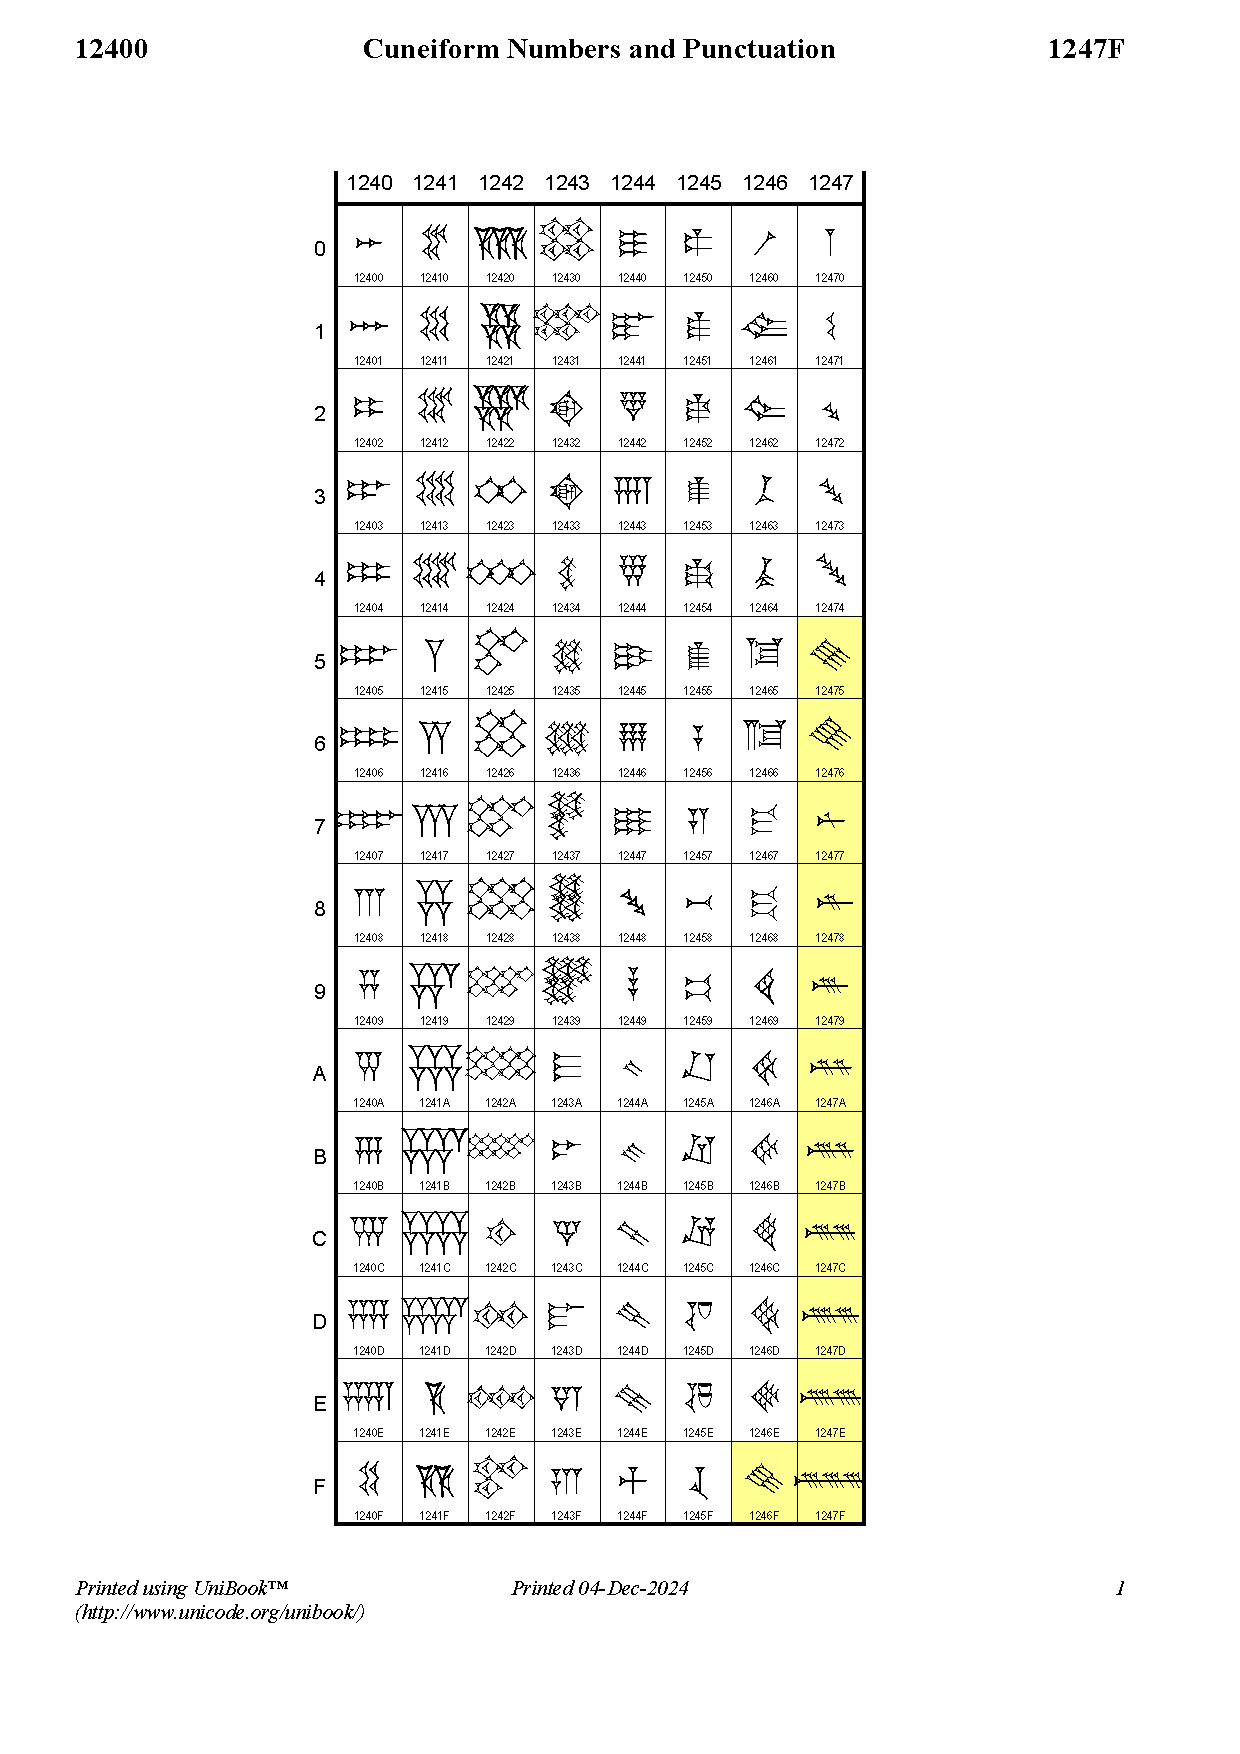
\includepdf[pages=-]{tenu-numerals-chart.pdf}
\subsection{Properties}
\label{properties}
Add to the respective UCD files the lines given in this section.
These are available as plain text files attached to this document.
Changes to derived files are not listed.
\fvset{fontsize=\scriptsize,breaklines,breaksymbol=\tiny\ensuremath{\textcolor{red}{\hookrightarrow}}}
\subsubsection{Name, General\_Category, Numeric\_Value, etc.}
%Attached: \textattachfile{tenu-numerals-ucd/UnicodeData.txt}{UnicodeData.txt}.
%\VerbatimInput{tenu-numerals-ucd/UnicodeData.txt}
\subsubsection{Line\_Break}
%Attached: \textattachfile{tenu-numerals-ucd/LineBreak.txt}{LineBreak.txt}.
%\VerbatimInput{tenu-numerals-ucd/LineBreak.txt}
\subsubsection{Script}
%Attached: \textattachfile{tenu-numerals-ucd/Scripts.txt}{Scripts.txt}.
%\VerbatimInput{tenu-numerals-ucd/Scripts.txt}
\subsubsection{Script\_Extensions}
%Attached: \textattachfile{tenu-numerals-ucd/ScriptExtensions.txt}{ScriptExtensions.txt}.
%\VerbatimInput{tenu-numerals-ucd/ScriptExtensions.txt}
\subsubsection{Block}
%Attached: \textattachfile{tenu-numerals-ucd/Blocks.txt}{Blocks.txt}.
%\VerbatimInput{tenu-numerals-ucd/Blocks.txt}

\section{DIŠ \emph{tenû} numerals}\label{dištenû}
This section discusses the following proposed characters:
\begin{itemize}[nosep]
  \item U+\textcsc{1246F} {\cuneiformComposite\sevenAshTenu} \textcsc{CUNEIFORM NUMERIC SIGN SEVEN ASH TENU}
  \item U+\textcsc{12475} {\cuneiformComposite\eightAshTenu} \textcsc{CUNEIFORM NUMERIC SIGN EIGHT ASH TENU}
  \item U+\textcsc{12476} {\cuneiformComposite\nineAshTenu} \textcsc{CUNEIFORM NUMERIC SIGN NINE ASH TENU}
\end{itemize}
\subsection{Name}
The existing numerals in the {\xsuxfont 𒀹} series are
named U+12039 {\cuneiformComposite 𒀹} \textcsc{CUNEIFORM SIGN ASH ZIDA TENU} for the first one
and U+\textcsc{1244A}–U+\textcsc{1244E} {\cuneiformComposite 𒑊}–{\cuneiformComposite 𒑎} \textcsc{CUNEIFORM NUMERIC SIGN $n$ ASH TENU} for the others.

Some\footnote{TODO also note gunû but contrast CROSSING rather than gi-li-mu-u, SQUARED rather than li-mu-bu i-gi-gu-ub-bu-u2} technical terms used in cuneiform character names are derived originate from the structural descriptions of
cuneiform signs by Akkadian-speaking scribes in late second and first millennium lexical texts.
[TODO(egg): Cite Yushu Gong on tenu itself]
In particular, the word \emph{tenû} is used to describe slanted signs or parts of signs:
thus {\xsuxfont 𒋙} is described as {\xsuxfont 𒁇} \emph{tenû} in \cite[\reverse i 46′]{P365233}\footnote{Note that
while the third millennium {\xsuxfont\addfontfeature{StylisticSet=1} 𒋙} and {\xsuxfont 𒁇} are related by a 45° rotation,
in the Neo-Assyrian style used by this list, these signs look like {\nafont 𒋙} and {\nafont 𒁇},
so that only one wedge is slanted, as noted in \cite[TODO]{Gong2000}.},
{\xsuxfont 𒃸} as {\xsuxfont 𒃷} \emph{tenû} in \cites[\reverse ii 47]{P391514}[\obverse ii 80]{P467315},
{\xsuxfont 𒄪} as {\xsuxfont 𒄩} \emph{tenû} in \cite[ii 33]{P391514},
{\xsuxfont 𒆿} as {\xsuxfont 𒆸} (containing) {\xsuxfont 𒀸} \emph{tenû} in \cite[\obverse 16′]{P365267}\footnote{TODO
something on spelling out names {\nafont 𒂵𒈾𒋼𒉡𒌑} \emph{ga-na te-nu-u₂} and {\nafont 𒊺𒋼𒉡𒌑} \emph{še te-nu-u}; \emph{ku te-nu-u}, etc.}.
In most cases, the direction of the slant not explicitly specified.
The terms \emph{kaba tenû} and \emph{zida tenû}, from Sumerian {\xsuxfont 𒆏} gab₂ ``left'' and {\xsuxfont 𒍣} zid ``right'' respectively,
are used in \cite{P345960}, which contrasts {\xsuxfont 𒀺} described as \emph{kaba tenû} and {\xsuxfont 𒀹} described as \emph{zida tenû}.

In modern transliteration, {\xsuxfont 𒀹} numerals are described as {\xsuxfont 𒀸} \emph{tenû} (ATF: \texttt{asz@t}) or {\xsuxfont 𒁹} \emph{tenû} (ATF: \texttt{disz@t}),
the latter being more common\footnote{For an example of a transliteration using aš tenû, see
\cite[§5.1.8 \reverse~1~4]{Greco2021}; note that only the HTML version uses aš tenû, the PDF uses diš.}.
% https://cdli.mpiwg-berlin.mpg.de/articles/cdlj/2021-2
Informative aliases using \emph{diš tenû} have been recommended for the existing characters in \cite{L2/24-239}.
The proposed names use ASH TENU for consistency with the already-encoded characters,
and the proposed annotations include informative aliases with \emph{diš tenû}.

\subsection{Ur III usage}
\begin{figure}
  \begin{center}
  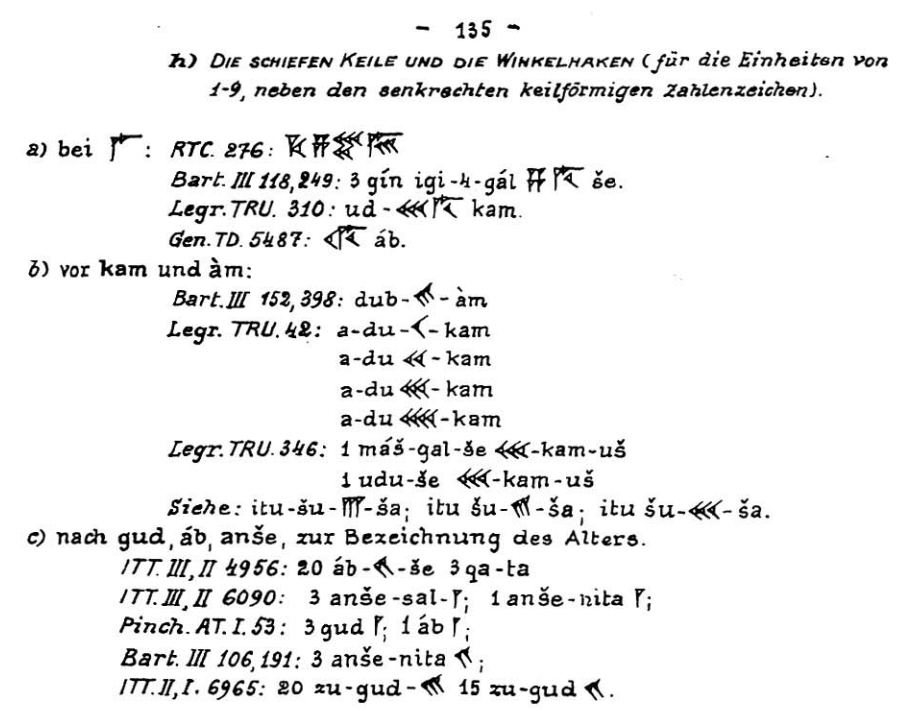
\includegraphics[width=0.75\textwidth]{kwu-p-135.png}
  \end{center}
  \caption{\cite[135]{KWU} \label{fig-KWU-135}}
\end{figure}
\begin{figure}
  \begin{center}
  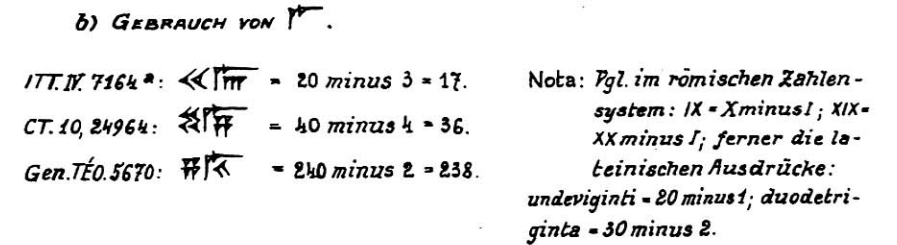
\includegraphics[width=0.75\textwidth]{kwu-p-132.png}
  \end{center}
  \caption{\cite[132]{KWU} \label{fig-KWU-132}}
\end{figure}
As described in \cite[135]{KWU} (see Figure~\ref{fig-KWU-135}),
slanted signs are used in Ur III economic texts primarily in
subtractive notation with {\xsuxfont 𒇲}\footnote{As noted in \cite[\pno~25 \withnote~40]{L2/24-210R},
the sign {\xsuxfont 𒇲} (lal, ``minus'')
is often ligated with the following numerals,
with the subtrahend placed under a sometimes considerably enlarged {\xsuxfont 𒇲},
similar to the layout of the radical in modern mathematical notation,
see, \exempligratia, \cite[\href{http://oracc.org/epsd2/P020092.69}{\reverse~3~1};
\href{http://oracc.org/epsd2/P020092.70}{2}]{P020092}.
The font used in this document ligates or kerns {\xsuxfont 𒀹} subtrahends,
but does not enlarge the {\xsuxfont 𒇲}.} lal\footnote{Also transliterated la₂, as in \cite{CDLI}.
In the transliterated Ur III corpus on \cite{CDLI}, out of 3304 occurrences of \texttt{(disz@t)},
1971 are in {\xsuxfont 𒇲$n$𒀹} \texttt{la2 $n$(disz@t)}.},
as well as for ordinals\footnote{1583 out of 3304 occurrences are {\xsuxfont $n$𒀹𒄰}
\texttt{$n$(disz@t)-kam}, including 647 after {\xsuxfont 𒇲}}
and for ages of animals in years\footnote{203 occurrences of
\texttt{gu4}, \texttt{ab2}, \texttt{ansze}, or \texttt{dur3} \texttt{$n$(disz@t)}}.

Accounts of animals giving their ages in years
rarely go beyond three-year old animals.
Subtractive notation, which appears in the ED IIIa period \cite[77]{Robson2008},
is used to compactly express numbers close to a larger round number, \exempligratia,
{\xsuxfont 𒌋𒇲𒀹} $10-1$ instead of {\xsuxfont 𒐎} for $9$,
{\xsuxfont 𒌍𒇲𒑊} $30-2$ instead of {\xsuxfont 𒎙𒐍} for $28$,
or {\xsuxfont 𒐕𒇲𒀹} $60-1$ instead of {\xsuxfont 𒐐𒐎} for $59$;
\confer{} IX instead of VIIII in Roman numerals.
It is therefore usually limited to small
subtrahends\footnote{Of the 1971 Ur III occurrences of
\texttt{lal $n$(disz@t)}, 1930 are with $n\leq2$,
of which 1823 with $n=1$.}.
Larger subtrahends do occur for quantities close to a much larger unit;
however in Ur III, they are often written {\xsuxfont 𒁹} numerals, as in
\cite[\obverse~2~15]{P109346} \smash{\xsuxfont 𒐉𒂆𒇲𒐌𒊺𒆬𒄀} ``$4$~shekels minus $7$~grains of gold'',
a weight which would otherwise be written
\smash{\xsuxfont 𒐈𒑛𒂆𒐐𒐈𒊺} ``$3+\frac{2}{3}$~shekels and $53$~grains'',
as $180\text{\xsuxfont 𒊺}=1\text{\xsuxfont 𒂆}$.

Ordinals with {\xsuxfont 𒀹} numerals are also typically limited to small numbers
or subtractive notation:
many of the attestations of {\xsuxfont $n$𒀹𒄰} ``$n$th''
are in year names\footnote{430 occurrences of \texttt{$n$(disz@t)-kam}
are on lines starting with \texttt{mu}, of which 308 are in {\xsuxfont 𒌋𒇲𒀹}.}, such as
{\xsuxfont 𒈬 𒃸𒄯𒆠 𒀀𒁺 𒑊𒄰𒀸 𒁀𒅆𒌨}
mu kar₂-ḫar\textsuperscript{ki} a-ra₂ $2${\xsuxfont 𒀹}-kam-aš ba-ḫul
``year Karhar was destroyed for the second time'' (31st year of Šulgi’s reign),
{\xsuxfont 𒈬 𒋛𒈬𒊒𒌝𒆠 𒀀𒁺 𒑋𒄰𒀸 𒁀𒅆𒌨} mu si-mu-ru-um\textsuperscript{ki} a-ra₂ $3${\xsuxfont 𒀹}-kam-aš ba-ḫul
``year Simurrum was destroyed for the third time'' (32nd year of Šulgi’s reign), or
{\xsuxfont 𒈬 𒋛𒈬𒊒𒌝𒆠 𒅇 𒇻𒇻𒁍𒌝 𒀀𒁺 𒌋𒇲𒀹𒄰𒀸 𒁀𒅆𒌨}
mu si-mu-ru-um\textsuperscript{ki} u₃ lu-lu-bu-um\textsuperscript{ki} a-ra2 $1${\xsuxfont 𒌋} lal $1${\xsuxfont 𒀹}-kam-aš
ba-ḫul ``year Simurrum and Lullubum were destroyed for the ninth time'' (44th year of Šulgi’s reign).
Larger ordinals are frequent, in particular for the day of the month, but these are written with
{\xsuxfont 𒁹} numerals, thus {\xsuxfont 𒌓𒐌𒄰} for ``the 7th day'' or {\xsuxfont 𒌓𒎙𒐍𒄰} for ``the 28th day''.

The rarity of the higher {\xsuxfont 𒀹} numerals in the Ur III corpus
likely explains the absence of $7${\xsuxfont 𒀹}--$9${\xsuxfont 𒀹}
from the répertoire of Unicode Version 5.0,
which was aiming to encode a répertoire appropriate for the Ur III period
and later.

\subsection{Early Dynastic usage}
The situation is different in the Early Dynastic corpus.
As described in \cite{L2/24-210R}, {\xsuxfont 𒀹} numerals are used in many
Early Dynastic metrological systems, and in particular in the Early Dynastic IIIb
length system
\newlength{\rodRopeWidth}
\settowidth{\rodRopeWidth}{$\underbrace{
  \text{\oneŊešʾuC}
  \xleftarrow{10}\text{\oneŊešTwoC}
  \xleftarrow{6}\text{\oneUC}}_{\text{\xsuxfont 𒃻𒁺}}=
  \underbrace{\text{\oneAšC}
  \xleftarrow{2}\text{\oneBanTwoC}}_{\text{\xsuxfont 𒂠}}$}
\begin{equation}
\begin{tikzcd}[row sep=tiny]
  \hspace*{\rodRopeWidth}
  \mathllap{\text{\xsuxfont 𒐕}
  \xleftarrow{\ \ \ 6\ \ \ }
  {\text{\xsuxfont 𒌋}}
  \xleftarrow{\ \ \ 2\ \ \ }\text{\xsuxfont 𒈦}}&
  \\
  &\arrow[lu, "10" above right, start anchor={west}, end anchor={east}]
  \arrow[ld, "10", start anchor={west}, end anchor={east}]\smash{\underset{\substack{\text{gi}\\\text{reed\vphantom{g}}\\3~\text{m}}}{\underbrace{\text{\xsuxfont 𒀹}}_{\text{\xsuxfont 𒄀}}}}
  \xleftarrow{\ \ 6\ \ }\smash{
    \underset{\mathclap{\substack{\text{kuš₃\vphantom{g}}\\\text{cubit\vphantom{g}}\\50~\text{cm}}}}
    {\underbrace{\text{\xsuxfont 𒀹}}_{\text{\xsuxfont 𒌑\vphantom{𒄀}}\mathrlap{*}}}}
    \xleftarrow{\ \ 3\ \ }\smash{
      \underset{\mathclap{\substack{\text{šu-du₃-a\vphantom{g}}\\\text{double-hand\vphantom{g}}\\17~\text{cm}}}}
      {\underbrace{\text{\xsuxfont 𒀹}}_{\mathclap{\text{\xsuxfont 𒋗𒆕𒀀\vphantom{𒄀}}*}}}}
    \xleftarrow{\ 10\ }\smash{
      \underset{\mathclap{\substack{\text{šu-si\vphantom{g}}\\\text{finger}\\17~\text{mm}}}}
      {\underbrace{\text{\xsuxfont 𒀹}}_{\mathclap{\text{\xsuxfont 𒋗𒋛\vphantom{𒄀}}*}}}}
  \\
  \underset{\substack{\text{\textsuperscript*{ninda}nindaₓ(DU)}\\\text{rod}\\6~\text{m}}}{\underbrace{
  \text{\oneŊešʾuC}
  \xleftarrow{10}\text{\oneŊešTwoC}
  \xleftarrow{6}\text{\oneUC}}_{\text{\xsuxfont 𒃻𒁺}}}=
  \underset{\substack{\text{eše₂}\\\text{rope}\\60~\text{m}}}
  {\underbrace{\text{\oneAšC}
  \xleftarrow{2}\text{\oneBanTwoC}}_{\text{\xsuxfont 𒂠}}}&
\end{tikzcd}
\tag{$L_{\text{ED IIIb}}$}
\label{systemLED}
\end{equation}
While these systems have a unit $1~\text{\xsuxfont 𒃻𒁺}=2~\text{\xsuxfont 𒄀}$,
lengths above $1~\text{\xsuxfont 𒄀}$ are only expressed in {\xsuxfont 𒂠},
or equivalently in tens of {\xsuxfont 𒃻𒁺}, and in
half-{\xsuxfont 𒂠} equal to $10~\text{\xsuxfont 𒄀}$.
We can therefore expect $7$--$9~\text{\xsuxfont 𒄀}$ to occur, expressed using
{\xsuxfont 𒀹} numerals.
Indeed, 37 texts in the transliterated ED IIIb corpus on \cite{CDLI}
contain undamaged attestations of either {\xsuxfont \sevenAshTenu 𒄀} or
{\xsuxfont \eightAshTenu 𒄀}\footnote{Of those, 34 have {\xsuxfont \sevenAshTenu 𒄀} and 9 have {\xsuxfont \eightAshTenu 𒄀}.};
some of these attestations are shown in Figures~\ref{figSevenReedsFirst}--\ref{figEightReedsLast}.
However, {\xsuxfont \nineAshTenu 𒄀} is not attested, since instead subtractive notation is used, as in
{\xsuxfont\threeŊešTwoC\fourUC\oneBanTwoC 𒇲𒀹𒄀} in \cite[\obverse~3~3]{P020129},
{\xsuxfont\oneŊešTwoC\fiveUC 𒃻𒁺𒇲𒀹𒄀𒌑𒑋} in \cite[\reverse~2~2]{P221272},
or {\xsuxfont 𒌋𒇲𒀹𒄀} in \cite[\obverse~3~8]{P020304}.

TODO something about sila, see P220703

The use of {\xsuxfont 𒀹} numerals for ordinals, especially for days,
is more prevalent in the Early Dynastic period
than in the Ur III period, and the use of subtractive notation is less frequent\footnote{Although
also attested, see, \exempligratia, \cite[\reverse~3~6]{P221346} {\xsuxfont 𒌓𒌋𒇲𒀹𒄰},
\cite[\reverse~2~1]{P221006} {\xsuxfont 𒀉𒌓𒌋𒇲𒀸𒄰}}.
in these numbers. We therefore find attestations of
{\xsuxfont\sevenAshTenu}--{\xsuxfont\nineAshTenu} in ``$n$th day'',
some of which are shown in Figures~\ref{figSeventhDay}--\ref{figNinthDay.}

In Ebla, the {\xsuxfont 𒀹} numerals are primarily used in subtractive notation,
see \cite[\pno~88 \withnote~298; \pno~120 \withnote~465; \pno~167 \withnote~739; \pno~180 \withnote~801]{Gori2024}.
However, contrary to Ur III, {\xsuxfont 𒀹} numerals remain used for large subtrahends,
thus \cite[\pno~101 \withnote~355]{Gori2024} cites occurrences of {\fourUC\xsuxfont 𒇲𒑌} for $36$ and
{\xsuxfont\oneAšC 𒇲𒑎𒈪𒀜}\footnote{Recall that {\xsuxfont 𒈪𒀜} \emph{mi-at} is Eblaite for ``hundred'',
see \cites[33]{Archi2015}[27]{L2/24-210R}.} for $94$.
In particular, \cite[129\psq]{Gori2024} cites occurrences of {\xsuxfont 𒇲$9$𒀹} in Ebla:
{\xsuxfont\oneUC 𒇲\nineAshTenu{} 𒈠𒈾 𒆬𒌓} ``$9$~minas and $51$~shekels of silver'' in
\cite[\href{http://ebda.cnr.it/tablet/view/1227\#47825}{\recto~1~1}]{P241283},
and {\xsuxfont \twoAšC 𒇲\nineAshTenu{} 𒈠𒈾 𒆬𒌓} ``$1$~mina and $51$~shekels of silver''
in \cite[\href{http://ebda.cnr.it/tablet/view/30\#6246}{\verso~3~2}]{P241325}.

\begin{figure}[H]
  \begin{center}
  \resizebox{.75\textwidth}{!}{
  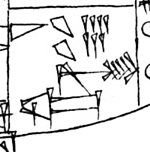
\includegraphics[height=17mm]{P221254 o 3 7 copy.png}
  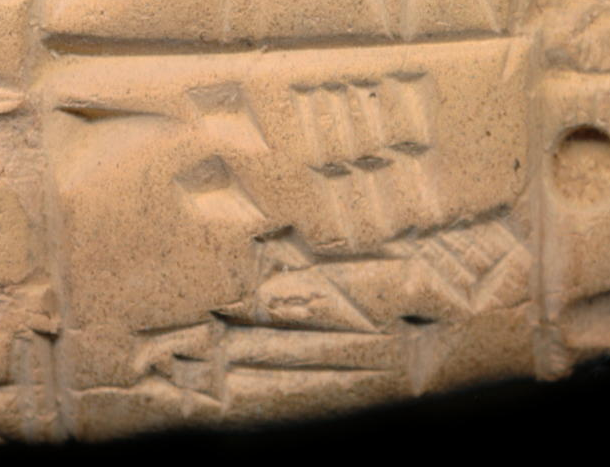
\includegraphics[height=17mm]{P221254 o 3 7.png}
  }
  \end{center}
  \caption[]{{\xsuxfont 𒐕𒎙\footnotemark\sevenAshTenu{}𒄀𒊕} ``$501$~m (first) width'' (of a field) in \cite[\obverse~3~7]{P221254} from Ŋirsu, dated to the reign of {\xsuxfont 𒌷𒅗𒄀𒈾}.
  Left: Copy from \cite{AllottedelaFuÿe1920}.
  Right: \cite{CDLI} photograph.}\label{figSevenReedsFirst}
\end{figure}
\footnotetext{TODO something about rhomboidal numerals, cite \cite{Gori2024}.}
\begin{figure}[H]
  \begin{center}
    \resizebox{.75\textwidth}{!}{
  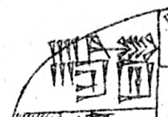
\includegraphics[height=17mm]{P221266 o 1 1 copy.png}
  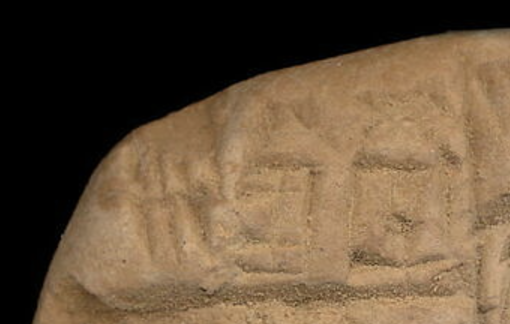
\includegraphics[height=17mm]{P221266 o 1 1.png}
  }
  \end{center}
  \caption{{\xsuxfont \sevenAshTenu{}𒄀 𒂊 𒆹} ``$21$~m of reed-bed dyke'' (attributed to {\xsuxfont 𒌨𒁮} the farmer) in \cite[\obverse~1~1]{P221266} from Ŋirsu, dated to the reign of {\xsuxfont 𒂗𒇷𒋻𒍣}. Left: Copy from \cite{AllottedelaFuÿe1920}.
  Right: \cite{LouvreCollections} photograph.}\label{figSevenReedsLast}
\end{figure}
\begin{figure}[H]
  \begin{center}
    \resizebox{.75\textwidth}{!}{
  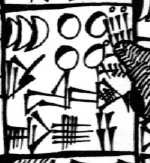
\includegraphics[height=17mm]{P020303 o 2 2 copy.png}
  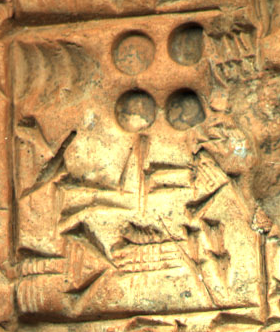
\includegraphics[height=17mm]{P020303 o 2 2.png}
  }
  \end{center}
  \caption{{\xsuxfont\threeŊešTwoC\fourUC 𒃻𒁺\eightAshTenu 𒄀 𒃴𒁉 𒌑𒑌} ``$1344$~m, its height $2$~m'' (dimensions of a dyke on the river {\xsuxfont 𒊊𒌉𒁕𒈿𒀀𒀭}) in \cite[\obverse~2~2]{P020303} from Ŋirsu, dated to the reign of {\xsuxfont 𒈗𒀭𒁕}. Left: Copy from \cite{Marzahn1991}.
  Right: \cite{CDLI} photograph.}\label{figEightReedsLast}
\end{figure}
\begin{figure}[H]
  \begin{center}
    \resizebox{.75\textwidth}{!}{
  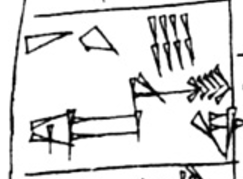
\includegraphics[height=17mm]{P221254 o 1 2 copy.png}
  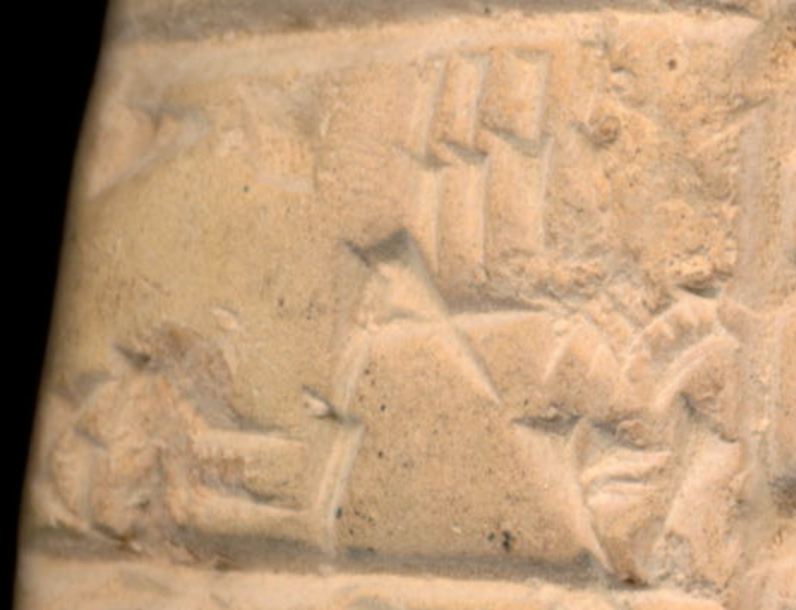
\includegraphics[height=17mm]{P221254 o 1 2.png}
  }
  \end{center}
  \caption{{\xsuxfont 𒐕𒌋\eightAshTenu{}𒄀𒊕𒁲} ``$444$~m equal widths'' (of a field) in \cite[\obverse~1~2]{P221254}.
  Left: Copy from \cite{AllottedelaFuÿe1920}. 
  Right: \cite{CDLI} photograph.}\label{figSevenReedsFirst}
\end{figure}
\begin{figure}[H]
  \begin{center}
    \resizebox{.75\textwidth}{!}{
  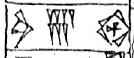
\includegraphics[height=17mm]{P220703 r 2 7 copy.png}
  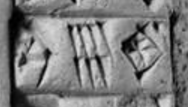
\includegraphics[height=17mm]{P220703 r 2 7.png}
  }
  \end{center}
  \caption{{\xsuxfont 𒌓\sevenAshTenu{}𒄰} ``seventh day'' in \cite[\reverse~2~7]{P220703} from Ŋirsu, dated to 3rd year of the reign of {\xsuxfont 𒈗𒀭𒁕}.
  Left: Copy from \cite{AllottedelaFuÿe1918}. 
  Right: \cite{LouvreCollections} photograph.}\label{figSeventhDay}
\end{figure}
\begin{figure}[H]
  \begin{center}
    \resizebox{.75\textwidth}{!}{
  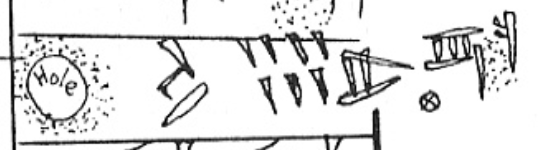
\includegraphics[height=17mm]{P221590 o 2 3 copy.png}
  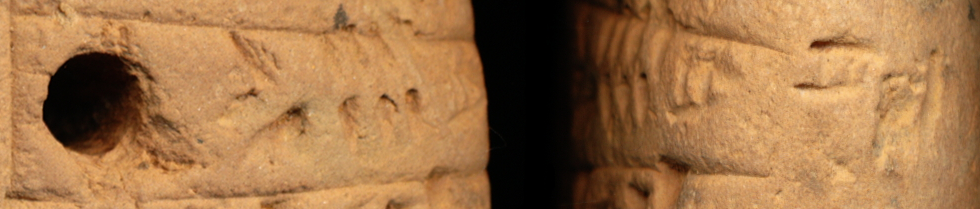
\includegraphics[height=17mm]{P221590 o 2 3.png}
  }
  \end{center}
  \caption{{\xsuxfont 𒌓\sevenAshTenu{}𒉌𒆷} ``seventh day passed'' in \cite[\obverse~2~3]{P221590} from Nippur.
  Left: Copy from \cite{Westenholz1975}. 
  Right: \cite{CDLI} photograph.}
\end{figure}
\begin{figure}[H]
  \begin{center}
    \resizebox{.75\textwidth}{!}{
  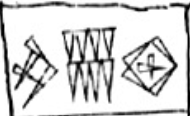
\includegraphics[height=17mm]{P220703 r 3 1 copy.png}
  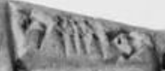
\includegraphics[height=17mm]{P220703 r 3 1.png}
  }
  \end{center}
  \caption{{\xsuxfont 𒌓\eightAshTenu{}𒄰} ``eighth day'' in \cite[\reverse~3~1]{P220703}.
  Left: Copy from \cite{AllottedelaFuÿe1918}. 
  Right: \cite{LouvreCollections} photograph.}\label{figEighthDay}
\end{figure}
\begin{figure}[H]
  \begin{center}
    \resizebox{.75\textwidth}{!}{
  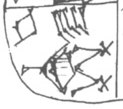
\includegraphics[height=17mm]{P222129 o 1 2 copy.png}
  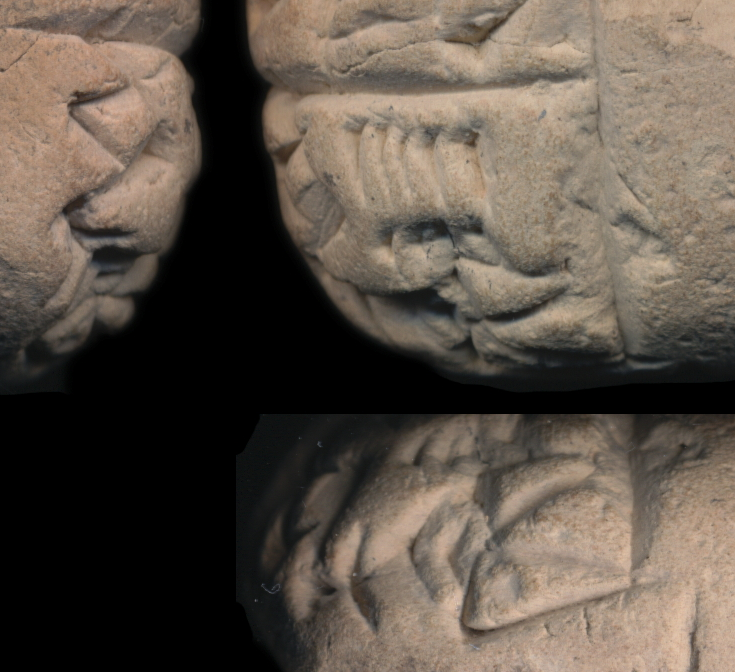
\includegraphics[height=17mm]{P222129 o 1 2.png}
  }
  \end{center}
  \caption{{\xsuxfont 𒌓\nineAshTenu{}𒆛} ``ninth day'' in \cite[\obverse~1~2]{P222129} from Šuruppag.
  Left: Copy from \cite{Martin2001}. 
  Right: \cite{CDLI} photograph.}\label{figNinthDay}
\end{figure}


\subsection{Stacking patterns}

\section{AŠ×(DIŠ \emph{tenû}) numerals}\label{aš×dištenû}

https://cdli.mpiwg-berlin.mpg.de/artifacts/452986/reader/209489
https://cdli.mpiwg-berlin.mpg.de/artifacts/467743/reader/213564

\subsection{Stacking patterns}

\begin{figure}[H]
  \begin{center}
  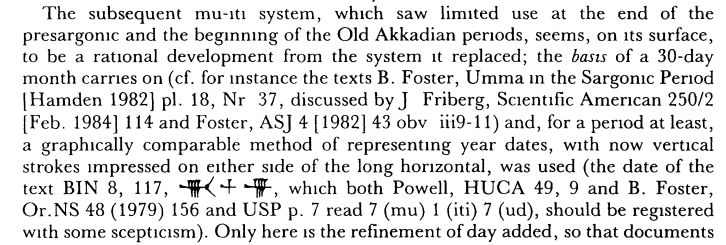
\includegraphics[width=0.75\textwidth]{eng88-p144-n17.png}
  \caption{TODO note that this should cite BIN 8, 116, not 117.}
  \end{center}
\end{figure}
\begin{figure}[H]
  \begin{center}
  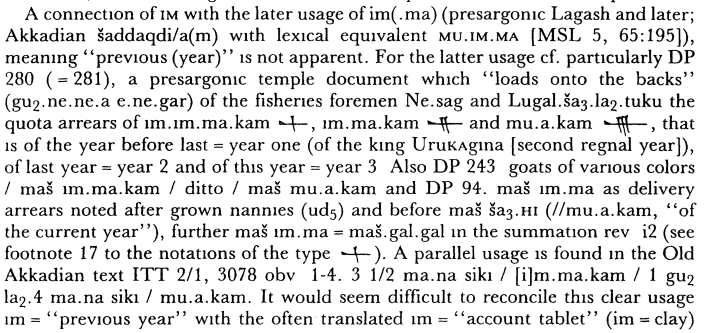
\includegraphics[width=0.75\textwidth]{eng88-p166-n37.png}
  \caption{TODO}
  \end{center}
\end{figure}

\section*{Acknowledgements}
\addcontentsline{toc}{section}{Acknowledgements}
% Peter Constable and Karljürgen Feuerherm provided useful feedback on the wording.
% Robin Leroy authored the bulk of the text.
% Rick McGowan suggested including a note in the character names list to clarify the identity of shrunk numerals in the code charts.
% Erica Scarpa brought the need for encoding the curviform numerals to our attention on multiple occasions and
% suggested several crucial references, most importantly \cite{Gori2023} which clearly demonstrates contrastive textual
% usage of curviform and cuneiform numerals in modern publications.
% Steve Tinney provided essential assistance on the interpretation of the Sumerian texts and suggested useful references.
% Ken Whistler gave important advice on matters of encodability, roadmapping, code point choice, and names list editing.

% The reference glyphs for most of the proposed characters whose Script\_Extensions value contains Pcun are based on a font
% made by Anshuman Pandey for \cite{L2/23-190}, itself based on designs by Bob Englund in \cite{archsigns}.
% The reference glyphs for \oneEighthIkuC{}, \oneBurʾuC{}--\fiveBurʾuC{}, and \oneBanTwoC{}--\fiveBanTwoC{}
% are based on designs by Steve Tinney.
% The glyphs were adjusted by Robin Leroy as described in §\ref{extraIdentity} and §\ref{stackingPatterns}.

% The Old Babylonian and Neo-Assyrian fonts used in §\ref{xsuxModel} and in the epigraphs in §\ref{metrology} and
% §\ref{non-numeric}
% are \emph{Santakku} and \emph{Assurbanipal},
% fonts created by Sylvie Vanséveren,
% available on the Hethitologie Portal Mainz \cite{Vanséveren2021}.
The \emph{CuneiformComposite} font by Steve Tinney is used when referring to the reference glyphs for already-encoded cuneiform.
\emph{Noto Sans Cuneiform}, by Monotype Imaging,
is used to for most of the cuneiform text in this document, with modifications (cuneiform glyph for {\xsuxfont 𒊹} ŠAR₂,
corrected glyps for {\xsuxfont 𒌦} UN and {\xsuxfont 𒌧} KALAM per \cite{Unicode16},
alternate glyph {\xsuxfont\addfontfeature{StylisticSet=1} 𒋙} for {\xsuxfont 𒋙}).
Arabic text is set in \emph{Scheherazade New} by SIL International;
Traditional Chinese text is set in \emph{Noto Serif TC} by Ken Lunde et al.;
monospace text is set in \emph{Consolas} by Luc(as) de Groot;
the remainder of the text is set in \emph{Cambria} and \emph{Cambria Math} by Monotype Imaging and Tiro Typeworks.
\printbibheading[heading=bibintoc]
\AtNextBibliography{\addfontfeatures{Numbers=Tabular}}
\printbibliography[heading=subbibintoc,title={Artefacts},type=artwork]
%\AtNextBibliography{\addfontfeatures{Numbers=Tabular}}
\printbibliography[heading=subbibintoc,title={ISO and Unicode documents},nottype=artwork,keyword=unicode]
\printbibliography[heading=subbibintoc,title={Online corpora and related projects},nottype=artwork,keyword=reference]
\printbibliography[heading=subbibintoc,title={Other documents},nottype=artwork,notkeyword=unicode,notkeyword=reference]
%\includepdf[pages=-2]{summary-form.pdf}
\end{document}